\chapter{Método}
\label{chapter:method}

Este capítulo descreve a elaboração de classificadores de sentimento de tweets
usando técnicas de processamento de linguagem natural e ciência de redes.
Serão detalhados as etapas de coleta de base de dados, as figuras de mérito
utilizadas nas avaliações dos modelos e o processo de treinamento dos
algoritmos.

\section{Bases de Dados}

Serão utilizadas duas bases de dados nesse trabalho, uma de treinamento e uma de
teste.
As bases serão formadas por tweets captados utilizando a
API~\footnote{https://developer.twitter.com/en/docs/twitter-api} do Twitter,
a qual fornece amostras de mensagens públicas, com a possibilidade de filtrar
pelas que contenham palavras-chave de interesse.

As mensagens de texto receberão alguns pré-processamentos antes de formarem as
bases de dados.
O primeiro passo será aplicar a tokenização, quebrando a mensagem em sequência
de palavras e removendo as pontuações.
Posteriormente as palavras serão postas em forma minúscula.
Por fim, menções a usuários e hiperlinks serão substituídos por tokens especiais.

Tendo objetivo de diminuir o custo de desenvolvimento do classificador textual será
adotado o método de anotação distante descrito por~\citet{go09} para formação da
base de dados de treinamento, usando emoticons como característica de anotação.
Serão selecionados manualmente emoticons positivos e negativos dentre os mais
frequentes nos textos captados.
As mensagens que possuírem um ou mais dos emoticons selecionados serão
categorizadas com a classe correspondente na base de treinamento.
Para remover possíveis ambiguidades, serão removidos da base os textos que
possuírem mais do que uma categoria.
Além disso, os emoticons utilizados na supervisão distante serão removidos dos
textos de treinamento para evitar a introdução de viés no classificador.

A base de testes será composta de tweets anotados manualmente.
Esta será utilizada para avaliar os modelos treinados com os métodos
semi-supervisionados.
Para esta finalidade, serão reservadas mensagens de um conjunto de usuários
selecionados aleatoriamente para compor essa base.
Esta separação é importante para evitar viés pois apesar de os métodos de
representação de usuários serem não supervisionados, como será descrito na
Seção~\ref{sec:development}, essa representação será utilizada no treinamento do
classificador.
As mensagens destes usuários serão disponibilizadas para anotação utilizando a
ferramenta Doccano~\footnote{https://github.com/doccano/doccano}.
Por fim, as mensagens anotadas comporão a base de dados de teste.

\section{Figuras de Mérito}

A avaliação dos algoritmos aplicados nestas bases será feita utilizando as figuras
de mérito descritas nessa seção.

Levando em consideração o desbalanceamento de classes das bases de dados não é
adequado a aplicação da acurácia pois esta favoreceria a classe majoritariamente
presente nas bases.
Como alternativa será adotada a área sob a curva ROC (\textit{receiver operating
characteristic}).
A curva ROC apresenta a relação entre probabilidade de detecção e falso alarme
para diferentes patamares de decisão de classificadores binários.
A área sob a curva ROC é uma medida que agrupa esse conjunto de taxas em um
número único, que representa o modelo em todos possíveis pontos de operação.

Como o objetivo abordado não apresenta um ponto de operação pré-definido, esse
também pode ser definido pela otimização de uma figura de mérito.
Desta forma, A seleção do limiar do classificador treinado será feita a partir do
índice SP~\cite{ciodaro12}.
Este índice consiste na média geométrica entre os pontos de média geométrica e
média aritmética entre a probabilidade de detecção da classe positiva $P_c$ e a
probabilidade de não obtenção de falso alarme $P_{nc}$, como mostra a
Equação~\ref{eq:sp}.

\begin{equation} \label{eq:sp}
    SP = \sqrt{\sqrt{P_c P_{nc}} \left(\frac{P_c + P_{nc}}{2}\right)}
\end{equation}

\section{Desenvolvimento}
\label{sec:development}

O objetivo deste trabalho é desenvolver classificadores de análise de sentimento
de tweets sem a necessidade de anotações de dados e que explorem a multimodalidade
do problema.
Desta forma, serão divididos os experimentos em duas etapas.
A primeira considerando apenas o texto das mensagens, serão avaliadas as técnicas
descritas no Capítulo~\ref{chapter:nlp}.
Posteriormente, serão utilizadas as representações das mensagens e as
representações da rede de usuários conjuntamente.
Desta forma analisaremos se a adição de informação do usuário infere em alguma
vantagem de performance no classificador.

\subsection{Classificadores de Processamento de Linguagem Natural}
\label{sec:nlp-classifier}

Seguindo os classificadores apresentados no Capítulo~\ref{chapter:nlp}, o
primeiro algoritmo aplicado será o Naïve Bayes.
As mensagens serão representadas por Bag-of-Words e, por isso, será utilizado
Naïve Bayes com distribuição multinomial.
Será utilizada a suavização de Laplace como regularizador do modelo.
O valor do parâmetro de suavização será selecionado de maneira a maximizar a
área sob a curva ROC (AUC).
A validação cruzada por K-partições servirá para maximizar esse valor, sendo
selecionadas 10 partições.

Posteriormente será treinado o classificador de SVM, também com representação de
Bag-of-Words.
Dado o grande volume de dados e a complexidade computacional será utilizado a
variação de SVM por método de gradiente como proposto por \citet{suykens99}.
Neste caso, será utilizada regularização $L_2$, assim como no classificador de
Naïve Bayes, este parâmetro será selecionado por validação cruzada de
K-partições de 10 partições, de maneira a maximizar a AUC.
Tanto o modelo de Naïve Bayes quanto o SVM foram treinados utilizando as
implementações disponibilizadas pela biblioteca Scikit-Learn~\cite{sklearn11}.

Para os modelos CNN e LSTM usaremos como representação o Word2Vec.
O treinamento do Word2Vec será feito a partir das mensagens amostradas do
Twitter, as mesmas mensagens utilizadas para formar a base de dados de treinamento
por supervisão distante, seguindo os mesmos pré-processamentos.
O modelo será treinado com o método \textit{continous bag-of-words} com
amostragem negativa de $5$ palavras, terá tamanho de janela de contexto $5$ e
dimensionalidade $100$ do vetor de representação.
O treinamento será feito utilizando a biblioteca Gensim~\cite{rehurek10}.

O treinamento dos classificadores de \textit{Deep Learning} por CNN e LSTM serão
treinados de formas similares.
Ambos terão como entrada os textos representados por Word2Vec.
Como as redes convolucionais dependem de tamanhos fixos de entrada, as mensagens
serão limitados a um tamanho máximo de \textit{tokens} definido pelo conjunto de
dados de treino.
As mensagens de tamanho menor que o tamanho máximo definido serão preenchidas
com vetores nulos.

Nesses classificadores, além das camadas convolucionais e LSTM, respectivamente,
uma camada será adicionada com um único neurônio para realização da
classificação.
Por serem modelos de alto custo computacional, não será realizada busca em
\textit{grid}.
Os hiperparâmetros selecionados foram baseados nos trabalhos apresentados no
Capítulo~\ref{chapter:nlp} que exploram o uso dessas técnicas em processamento
de texto.
A rede convolucional será composta por três camadas convolucionais em paralelo,
cada uma como 100 filtros convolucionais com tamanhos respectivamente de 3, 4 e
5 tokens.
O classificador de LSTM, por sua vez, conterá duas camadas bidirecionais em
série de 100 neurônios cada.
Ambos os modelos utilizaram \textit{dropout} durante o treinamento com
probabilidade de 50\% de desligamento do neurônio e regularização L2 de fator
$10^-3$.
Serão realizados $10$ treinamentos de cada modelos, dado que o treinamento de
redes neurais é propenso a estagnar em mínimos locais.
Como estes métodos tem alto custo computacional, não será utilizada a validação
de K-partições.
Será selecionado aleatoriamente um conjunto de validação composto por 20\% dos
dados de treinamento, sendo este usado para seleção dos hiperparâmetros.
Para reduzir o efeito de \textit{overfitting} será aplicado o \textit{early
stopping}.

Por fim, será avaliada a representação de palavras pela técnica ELMo.
Como este modelo contêm um número elevado de parâmetros, será utilizado um
conjunto de pesos pré-treinados~\footnote{https://allennlp.org/elmo}, os quais
foram treinados em textos em português retirados da
Wikipédia~\footnote{https://www.wikipedia.org}.
O modelo gera vetores de representações de tamanho $1024$ e foi treinado com
duas camadas.
Será utilizada apenas a camada superior do modelo, dado que para tarefa de
análise de sentimento se faz mais relevante a informação semântica das mensagens.
Em conjunto com essa representação, será utilizado o modelo de CNN para
classificação do texto.
Este seguirá o mesmo método do anterior, limitando as mensagens em tamanho,
preenchendo com vetores nulos e otimizando hiperparâmetros por busca em
\textit{grid}.

Em virtude do alto custo computacional do modelo BERT apresentado no
Capítulo~\ref{chapter:nlp} não será possível o treinamento do mesmo para
comparação, apesar dos bons resultados obtidos em seu artigo de referência.

Dessa forma se concluirá a comparação de desempenho dos algoritmos clássicos
de processamento de linguagem natural com as técnicas neurais desenvolvidas no
decorrer da última década.
Neste estágio foram analisadas apenas os dados textuais das mensagens, a seguir
será apresentado o método que unificará a informação provinda dos textos com as
informações obtidas do usuário.

\subsection{Classificadores Multimodais}
\label{sec:multimodal-classifier}

% TODO: mini introducao falando dos metodos conjuntos

A primeira etapa para formação dos classificadores multimodais é o treinamento
não-supervisionado das representações de usuário.
Serão empregadas 3 das técnicas apresentadas no Capítulo~\ref{chapter:networks},
uma de cada um dos tipos de modelos.
O grafo formado será homogêneo em que os usuários são codificados como vértices
e os \textit{retweets}, operação de compartilhamento de uma mensagem de outro
usuário, formam uma aresta direcional entre ambos.

% TODO: retirar parte que cabe no resultados
A rede obtida é formada por aproximadamente $5,5$ milhões de nós e $28$ milhões
de arestas.
Como elucidado no Capítulo~\ref{chapter:networks}, a maioria dos algoritmos de
representação de vértices tem grandes requisitos de memória.
Portanto, algumas restrições foram necessárias para viabilizar o treinamento dos
modelos.
Cada modelo tem sua limitação própria, mas será seguida a mesma estratégia para
atacar esse problema.
O grafo original será reduzido para o subgrafo composto pelos nós da maior
componente fortemente conexa, ou seja, o maior subgrafo em que todos os nós
apresentam caminhos entre si.
% TODO: preencher valor
Este procedimento reduz o grafo a um total de $x$ vértices e $y$ arestas.
Ainda assim, nos casos em que esta rede ainda seja grande demais para viabilizar
o treinamento, serão selecionados aleatoriamente vértices, garantindo apenas que
os vértices presentes na base de teste estejam incluídos na rede a ser treinada.
Para facilitar a comparação, todas as técnicas usaram o mesmo tamanho de
\textit{embedding}.

O primeiro método para representação dos vértices avaliado será será o modelo de
fatoração matricial \textit{Locally Linear Embedding}.
Este utiliza a matriz de adjacência para criar representações que aproximem nós
vizinhos.

Em seguida, será aplicado o \textit{Node2Vec} como representante dos algoritmos baseados
em passeios aleatórios.
Este será treinado com parâmetros fixos.
Os valores de $p$ e $q$ serão $1$.
Os passeios aleatórios terão $80$ passos e serão realizados $10$ inicializações
aleatórias por cada nó.
O treinamento usará janelas de contexto de tamanho $10$ e serão treinados por
$3$ épocas.

Por fim, será avaliado o método de redes convolucionais aplicadas a grafos.
Como o modelo GCN é um modelo supervisionado, será aplicado a técnica Graph
Infomax para treinamento não-supervisionado.
Outra adaptação necessária é que enquanto os outros métodos dependem apenas da
estrutura da rede, o GCN usa também características dos vértices para
treinamento da representação.
Se tratando de redes sociais há várias possibilidades de característica para ser
exploradas como número de contatos, descrição do perfil, foto, entre outras.
Entretanto, essas abordagens não serão exploradas nesse trabalho, usaremos como
característica o grau do nó na rede.

Desta forma, haveremos treinado os classificadores textuais e as representações
dos usuários, restando portanto a testar se a combinação dos mesmos dos mesmos
infere em algum aumento de performance.
Serão retirados os neurônios da última camada, a camada de classificação, dos
modelos de CNN e LSTM já treinados.
Serão concatenadas as camadas restantes dos modelos textuais com as
representações de usuários e adicionada uma nova camada de classificação.
A figura~\ref{fig:network_composition} demonstra a arquitetura final resultante
da composição dos dois classificadores.
O modelo será treinado novamente nos dados anotados por supervisão distante, com
os pesos inicializados pelos modelos pré-treinados.
Concluindo-se, portanto, o conjunto de experimentos realizados nesse trabalho.

\begin{figure}[h]
\begin{center} {
    \begin{center}
    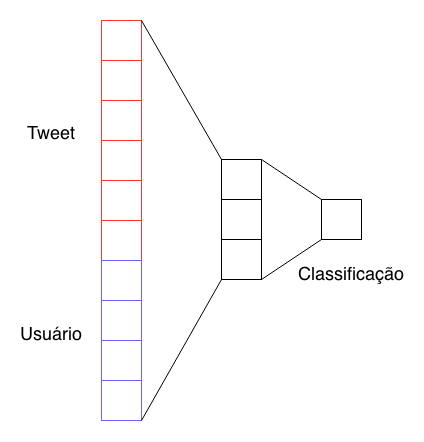
\includegraphics[scale=0.45]{images/network_composition.png}
    \caption{Arquitetura composto pela combinação de classificadores de
        informação textual e de usuário concatenados. Adicionou-se também uma
        camada de neurônios que será treinado para combinar as representações.}
    \label{fig:network_composition}
    \end{center}
}
\end{center}
\end{figure}
